%BEGIN JC
%\subsection{Isosurface Contouring}
After obtaining the optimized voxel data, the next step is to generate a \emph{mesh based
geometry}, which is a mesh representation of the volume data.  
This will be used in conversion of our surface back to CAD format, in particular, to NURBS representation. In order to achieve it, the
data will be represented by a contour of a smooth function, rendering an isosurface. Based on the algorithm used, the mesh can be composed of triangles or quadrilaterals, also known as quads. A well-know approach to tackle this problem is the \emph{Marching Cubes} technique.


\subsubsection{Marching Cubes} 
%\subsection{Marching Cubes} 
\begin{figure}
\centering
   \scalebox{0.8}{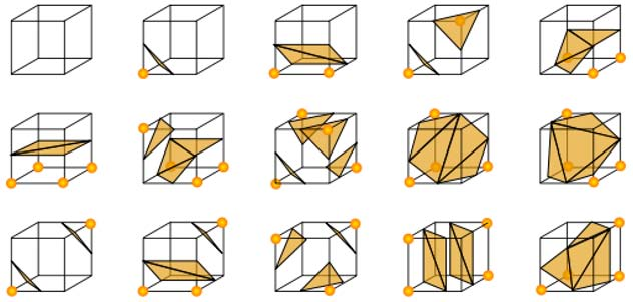
\includegraphics{Pictures/cubes.pdf}}\\
   \caption{Base cases of Marching Cubes. Figure taken from \cite{Marching2006} }
   \label{fig:MC_basecase}
\end{figure}
The \emph{Marching Cubes} algorithm \cite{Marching2006} takes as an input a regular volumetric data set and extracts a mesh. It
divides the space into cubes, which are defined by the volume information. Each cube has scalar
information on its vertices, the value is equal or above a marked isovalue. Therefore each of the
eight vertices of a cube can be marked or unmarked. According to these values vertices are drawn
on the edges of the cube at calculated points with the use of interpolation. 

By connecting the vertices we obtain a polygon on each cube. There are 256 possible cases. Many of these can be constructed by rotating or reflecting of previous cases.  Therefore  
there are 15 base cases which represent all the possibilities of the marching cubes (see \autoref{fig:MC_basecase}). 
The original algorithm presents two main problems. First, it does not guarantee neither
correctness nor topological consistency, which means that holes may appear on the surface due
to inaccurate base case selection. Second, another problem is ambiguity, which appears when two
base cases are possible and the algorithm chooses the incorrect one. There are many extended Marching Cubes
algorithms that tackle the problems of the original one, getting rid of the ambiguities and
providing correctness.  

%\subsection{Dual Contouring}
\subsubsection{Dual Contouring}
The idea of the \emph{Dual Contouring} algorithm is similar to Marching Cubes, but instead of generating vertices on the
edges of the cubes, it locates them inside the cube. \autoref{fig:bunny_MCDC} shows the basic differences in both approaches.
The vertices associated with the four contiguous cubes are joined and form a quad. The question now is
which place inside the cube is the ideal one to insert each vertex. Different dual algorithms are classified 
according to the answer for this question. Dual Contouring in particular generates a vertex positioned at the minimizer of a
quadratic function which depends on the intersection points and normals. Therefore the method needs Hermite 
data (exact intersection of points and normals) to work with. 
The quadratic function is defined in \cite{Hermite2002} as follows:
\begin{equation*}
E(x)= x^TA^TAx-2x^TA^Tb+b^Tb
\end{equation*}
Where \textit{A} is a matrix whose rows are the normals and \textit{b} is a vector whose entries are the product of normals and intersection points. To solve this system, a numerical treatment is needed. As proposed in \cite{Hermite2002} one approach is to compute the
singular value decomposition of \textit{A} and form the pseudo-inverse by truncating its small singular values. 
%1=Dual Contouring of HErmite DAta


The main advantage of this method over MC is the acquisition of better aspect ratios. On the other hand the need of Hermite Data
represents a disadvantage. Furthermore, there is no open source algorithm that implements the Dual Contouring scheme.

%\subsection{VTK Toolbox}
%\subsubsection{Installing VTK}
%VTK was installed using the Linux platform with pre-installed gcc. VTK offers the possibility to use Python, TLC or C++ for
%development. VTK toolbox is actually a C++ library, which is implemented in other languages. We
%decided to continue the project with C++ since it gives the possibility to explore the original code.
%%A few dependency problems were encountered, nevertheless they were easy to track back. If any
%problems were to be found at installation time, please refer to the VTK Wiki where the procedure
%is explained step by step.


%\subsubsection{Implementing the VTK Classes}
%\subsection{VTK Toolbox}
\begin{figure}
\centering
   \scalebox{0.35}{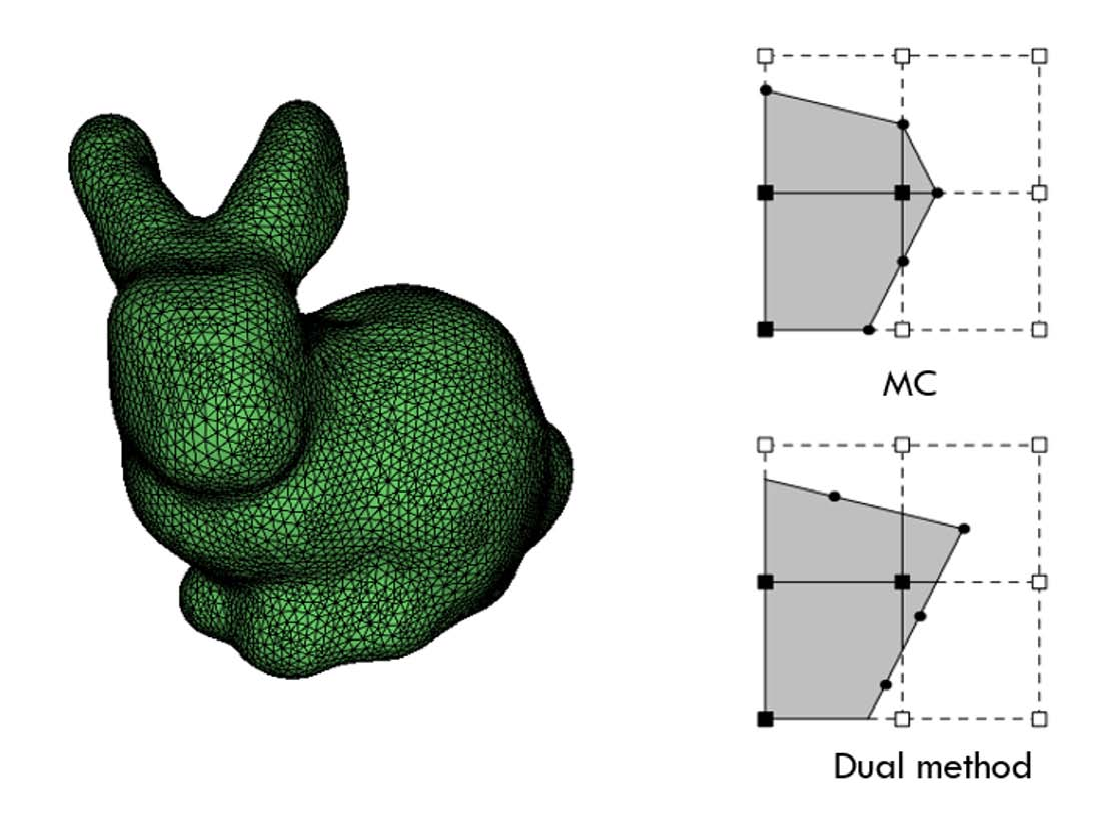
\includegraphics{Pictures/bunny_MC.pdf}}\\
   \caption{\textit{Left:} The famous Stanford Bunny after application of Marching Cubes. \textit{Right:} Main difference between MC and Dual methods.  Figures taken from \cite{Hermite2002} }
   \label{fig:bunny_MCDC}
\end{figure}
%The VTK toolbox was used in order to implement the algorithms on our optimized data. It is a heavily object
%oriented toolbox. Our first approach was to use the built in Marching Cubes algorithm,
%nevertheless it did not work with our unstructured grid data. It just works for ImageData and
%PolyData . For structured and unstructured grids the tool to render the isosurface is the \textit{Contour Filter} tool. Unfortunately the documentation does not present which algorithm the tool uses. It
%can be inferred that it is an extended Marching cubes algorithm.



%It finally allowed visualization but it created one problem. Holes are lost in
%the process.




%%%%%% THIS PART WILL BE INCLUDED IN THE NEXT M. in case this approach is needed.

%\subsection{Voxel Data to NURBS}
%There are two possible roads to go from the voxel data to the CAD representation (in our case NURBS based representation).
%\subsubsection{Quad Contouring}
%This approach uses the Dual Contouring algorithm as first step in order to obtain a quad mesh
%representation from the voxel data. The first challenge is to implement the algorithm
%with the ideas presented in \cite{Hermite2002} correctly. The original Marching Cubes algorithm is
%implemented in VTK but the source code is not public. Once this first step is done, the quads will be chosen for the
%NURBS parametrization. A second step considers multiple smaller quads which have to be
%combined into one larger patch. This is another challenge, since the remeshing of quad meshes
%is not as straightforward as with the triangles. Different approaches have been taken in order to achieve this coarsening. In \cite{Puppo2010} an incremental and greedy approach, which is based on local operations only, is presented. It depicts an iterative process which performs local optimizing, coarsening and smoothing operations. Other approaches, like the one presented in \cite{Dong2005} uses smooth harmonic scalar fields to simplify the mesh.

%2= “Practical quad mesh simplification”
%3= “Harmonic Functions for Quadrilateral Remeshing of Arbitrary Manifolds”


%\subsubsection{Multiresolution Analysis of Arbitrary Meshes}
%With \textit{Multiresolution Analysis of Arbitrary Meshes} approach there is no need to apply a Dual Contouring algorithm, since it takes as
%beginning data the triangles from the Marching Cubes. The main concepts are shown in the paper \cite{eck1996automatic}. It mainly takes a series of intermediate steps which permits a parametrization of data. It includes a partitioning scheme based on the ideas of the Voronoi Diagrams %reference
 %Delaunay triangulations %reference
. %Large patches or quads are obtained with this method. 

%4=reference to MAAM, a.k.a Benni's favorite paper!

%%implementation part!
%Both approaches have not been implemented in open source documentation, therefore there is a need to implement it from scratch. Up to now, the second approach has been chosen.

%END JC
